% !TEX root = ../The-Haptic-Printer.tex
%
\chapter{Literature Survey}
\label{sec:related}

Once our project objective was clear we had to find out existing rendering techniques available for Ultrahaptics device. Also, we had to look into Ultrahatics Software Development Kit (SDK) and the available Application Program Interface (API) so that the application can be developed. After referring to Ultrahaptics SDK we came to know that there are two techniques available to develop our application, namely Amplitude Modulation (AM) and Time Point Streaming(TPS). To further understand these topics we had to look into the concepts and working of these techniques. So we did a literature survey and in the further subsection we have listed our key findings and short explanation of both the techniques.

\begin{figure}[htb]
	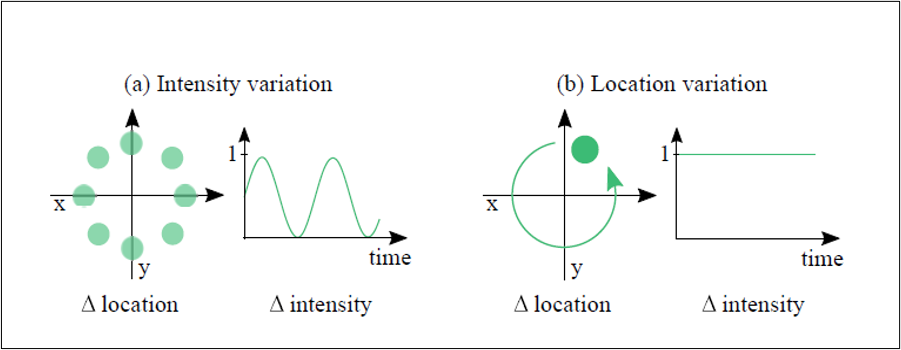
\includegraphics[width=\textwidth]{gfx/am_tps.png}
	\caption{(a) shows working of Amplitude Modulation technique (b) shows working of Spatiotemporal Modulation technique \cite{Frier2018}}
	\label{fig:related:am_tps}
\end{figure}

\section{Amplitude Modulation}
\label{sec:related:sec1}

In amplitude modulation technique, the ultrasound waves emitted by the phased arrays and are modulated by switching them off and then on again fast enough to stimulate the vibration-sensitive touch receptors (mechanoreceptors) in the skin of the hands, giving tactile sensation. But these switching on and off of waves are not so easily perceived by the user as the frequencies are in the range of 40Hz to 400Hz. In order to smoothen out this effect the ultrasound is modulated with a sinusoidal wave.\cite{am}

As shown in Fig 2.1 (a) the control points have varying intensity emitted by the device which creates pressure points on user's palm. Using this technique, we can render shapes by updating the coordinates of  the shape rapidly. Also, we can use one more technique here by emitting multiple control points at the same time to complete the shape outline.


\section{Spatiotemporal Modulation}
\label{sec:related:sec2}

Spatiotemporal Modulation also called as time point streaming is a technique where we rapidly move the control point emitted by the device along the shape outline to create tactile sensation. Here the control point can be fixed to a same intensity level or we can use any sine or cosine wave as intensity values for varying intensities.\cite{tps} 

As shown in Fig 2.1 (b) the control point moves rapidly along the circle shape outline with constant intensity. 

Once we discovered the various techniques available in Ultrahaptics SDK we decided to go ahead with these two techniques. There are several tweaks available to these two techniques which can also be used for rendering. However, due to the limitation of available Ultrahaptics SDK API we chose to stick to these two techniques.  

